% Asset ID: FA22SamplingAndEstimationTikZ-001
% Asset type: TikZ diagram
% Unit: FA22 – Further A2 2 Applied Mathematics
% Topic code: FA22-EST
% Purpose: Standard normal curve with central 95%, 2.5% tails and z = ±1.96.
\documentclass[tikz,border=8pt]{standalone}
\usepackage{amsmath}
\usepackage{xcolor}
\usetikzlibrary{arrows.meta}
\definecolor{Canvas}{HTML}{FAF9F6}
\definecolor{Ivory}{HTML}{FFFFF0}
\definecolor{LineSoft}{HTML}{E5E5EA}
\definecolor{Gold}{HTML}{C5A059}
\definecolor{GoldDeep}{HTML}{D4AF37}
\definecolor{Blush}{HTML}{FBEFEF}
\definecolor{Ink}{HTML}{2C2C2E}
\begin{document}
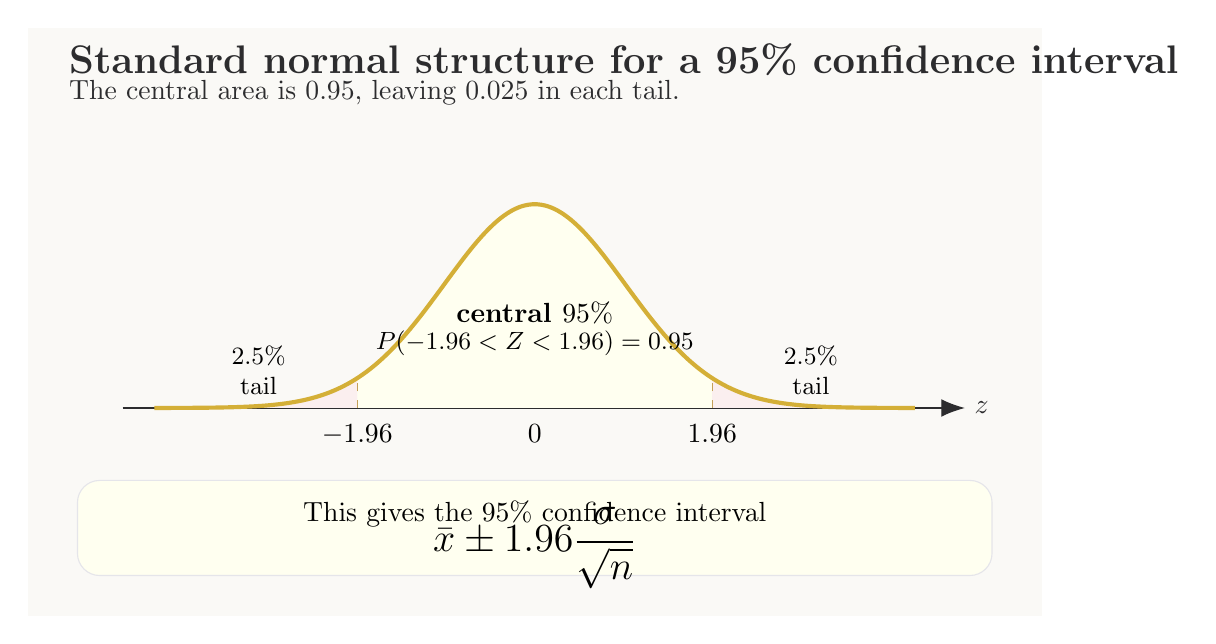
\begin{tikzpicture}[x=1.15cm,y=1.15cm]
\fill[Canvas] (-5.6,-2.3) rectangle (5.6,4.2);
\node[anchor=west, text=Ink, font=\bfseries\Large] at (-5.25,3.85){Standard normal structure for a 95\% confidence interval};
\node[anchor=west, text=Ink] at (-5.25,3.48){The central area is \(0.95\), leaving \(0.025\) in each tail.};
\draw[Ink, -{Latex[length=3mm]}] (-4.55,0) -- (4.75,0) node[right] {\(z\)};
\fill[Blush] plot[domain=-4.2:-1.96, samples=80, smooth] (\x,{2.25*exp(-0.5*\x*\x)}) -- (-1.96,0) -- (-4.2,0) -- cycle;
\fill[Ivory] plot[domain=-1.96:1.96, samples=120, smooth] (\x,{2.25*exp(-0.5*\x*\x)}) -- (1.96,0) -- (-1.96,0) -- cycle;
\fill[Blush] plot[domain=1.96:4.2, samples=80, smooth] (\x,{2.25*exp(-0.5*\x*\x)}) -- (4.2,0) -- (1.96,0) -- cycle;
\draw[GoldDeep, line width=1.5pt] plot[domain=-4.2:4.2, samples=180, smooth] (\x,{2.25*exp(-0.5*\x*\x)});
\draw[Gold, dashed] (-1.96,0) -- (-1.96,{2.25*exp(-0.5*1.96*1.96)});
\draw[Gold, dashed] (1.96,0) -- (1.96,{2.25*exp(-0.5*1.96*1.96)});
\node[below] at (-1.96,-0.08) {\(-1.96\)};
\node[below] at (1.96,-0.08) {\(1.96\)};
\node[below] at (0,-0.08) {\(0\)};
\node[font=\bfseries] at (0,1.05) {central \(95\%\)};
\node[font=\small] at (0,0.72) {\(P(-1.96<Z<1.96)=0.95\)};
\node[font=\small,align=center] at (-3.05,0.42){\(2.5\%\)\\tail};
\node[font=\small,align=center] at (3.05,0.42){\(2.5\%\)\\tail};
\draw[LineSoft, rounded corners=8pt, fill=Ivory] (-5.05,-1.85) rectangle (5.05,-0.8);
\node at (0,-1.17){This gives the 95\% confidence interval};
\node[font=\Large] at (0,-1.55){\(\displaystyle \bar{x}\pm 1.96\frac{\sigma}{\sqrt{n}}\)};
\end{tikzpicture}
\end{document}
